\section{Relación}
\label{sec:relacion}

En las \texttt{Secciones \ref{sec:atributo}}, \texttt{\ref{sec:metodo}} y
\texttt{\ref{sec:clase}} se definieron los componentes clave que permiten
sistematizar la generación de código para los componentes base de los
diagramas de clase, en ésta sección, se describe un componente que permite
la asociación de diferentes clases dentro de un modelo, una \texttt{Relación}.

Estas relaciones permiten la asociación entre dos clases. Director permite
definir una sección en la cual se pueden definir un conjunto de relaciones que
luego se tendrán en cuenta a la hora de generar los componentes que se
definieron en el modelo.


\subsubsection{Analizador Léxico}
Primeramente se definen los patrones que ayudan al lenguaje a identificar los
direfentes componentes léxicos del lenguaje, para un mejor entendimiento de los
patrones que se describen mediante expresiones regulares (y es de público
conocimiento que son complicados de leer), se va a separar este componente
\texttt{relacion} en partes mas pequeñas para poder entender de manera más
sencilla la expresión, estas partes serán:
\begin{itemize}
  \item Nombre de clase (+Rol) [\texttt{Fragmento \ref{rerenomclase}}]
  \item Cardinalidad [\texttt{Fragmento \ref{rerecard}}]
  \item Tipo de relación [\texttt{Fragmento \ref{reretiprel}}]
\end{itemize}

y para finalizar se presenta la expresión regular en donde todos las partes
están unidas

\begin{lstinputlisting}[basicstyle=\footnotesize\ttfamily, caption={Regex -
  Nombre clase (+Rol) [Relación]},
  label=rerenomclase]{regex/relacion/rol_asociacion.txt}


\begin{lstinputlisting}[basicstyle=\footnotesize\ttfamily, caption={Regex -
  Cardinalidad [Relación]}, label=rerecard]{regex/relacion/cardinalidad.txt}

\begin{figure}[H]
	\centering
	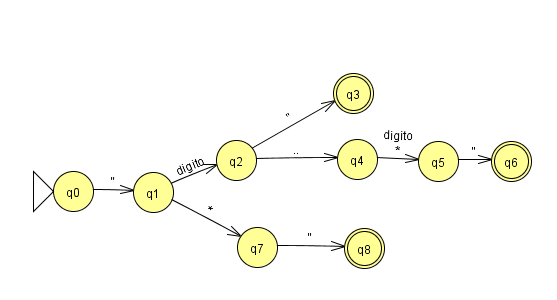
\includegraphics[width=.7\linewidth]{automatas_finitos/cardinalidadDrt.png}
	\caption{Autómata finito - Cardinalidad para una Relación}
	\label{fig:af_relacion_cardinalidad}
\end{figure}

\begin{lstinputlisting}[basicstyle=\footnotesize\ttfamily, caption={Regex -
  Tipo de Relación [Relación]},
  label=reretiprel]{regex/relacion/tipo_relacion.txt}

\begin{figure}[H]
	\centering
	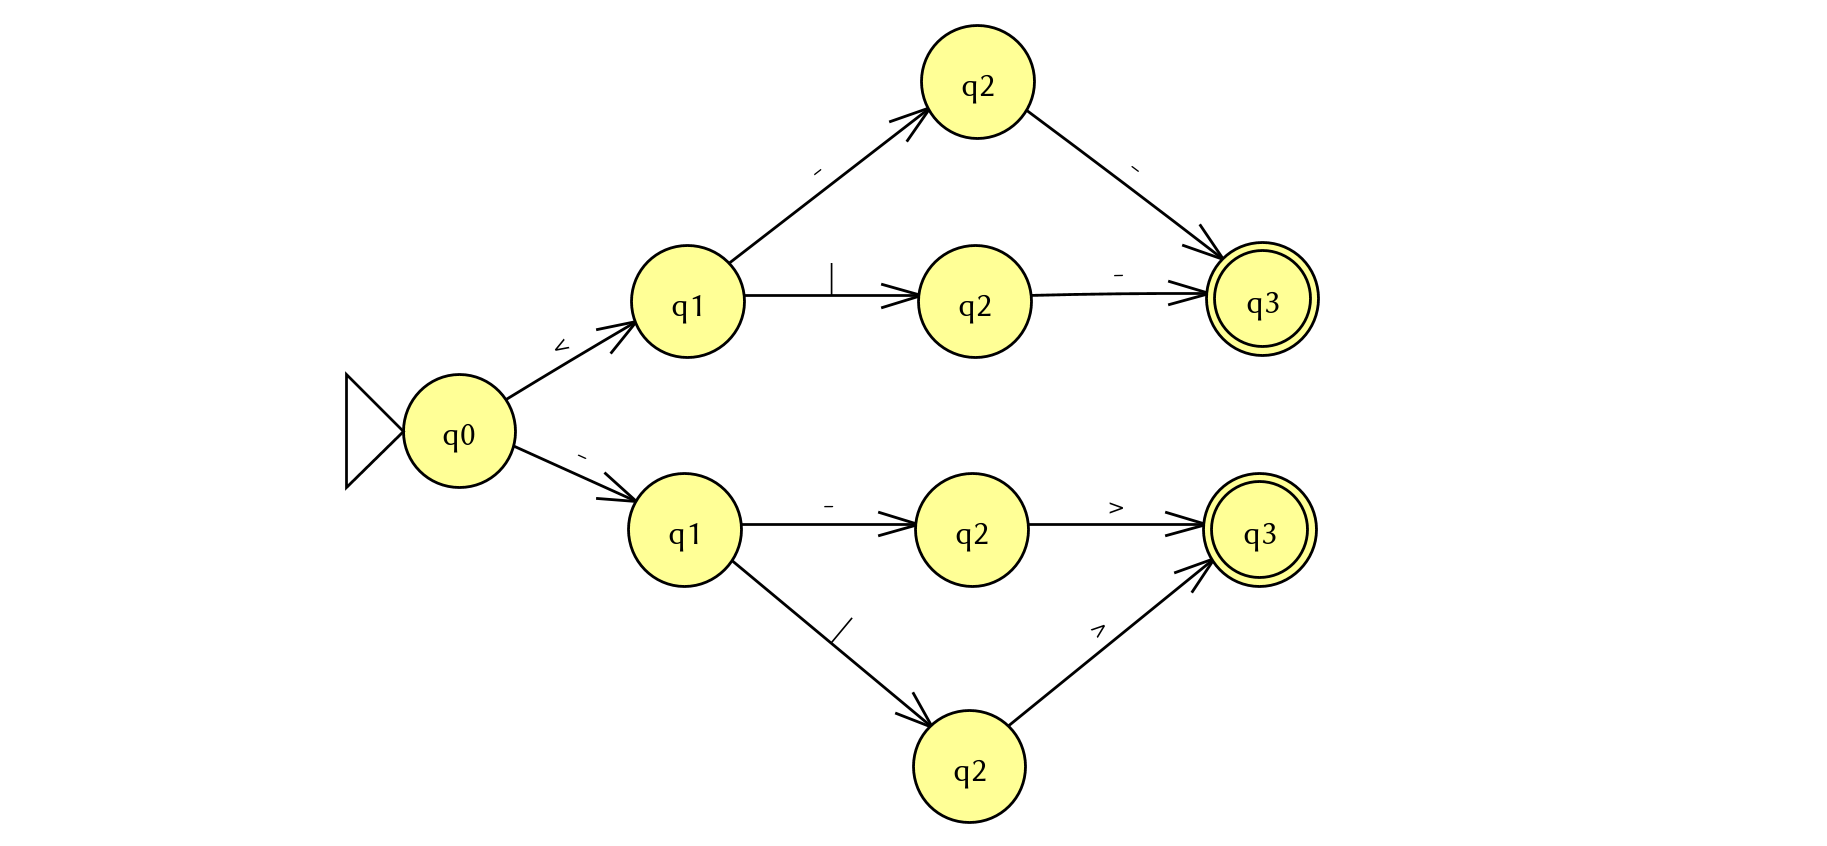
\includegraphics[width=.7\linewidth]{automatas_finitos/tipo-relacion.png}
	\caption{Autómata finito - Tipos de Relación}
	\label{fig:af_tipos_relaciones}
\end{figure}

Y finalmente, se tiene la expresión para los patrones en una sola expresión
  regular:

\begin{lstinputlisting}[basicstyle=\footnotesize\ttfamily, caption={Regex -
  Relacion},
  label=rerelacion]{regex/relacion/relacion.txt}

\begin{figure}[H]
	\centering
	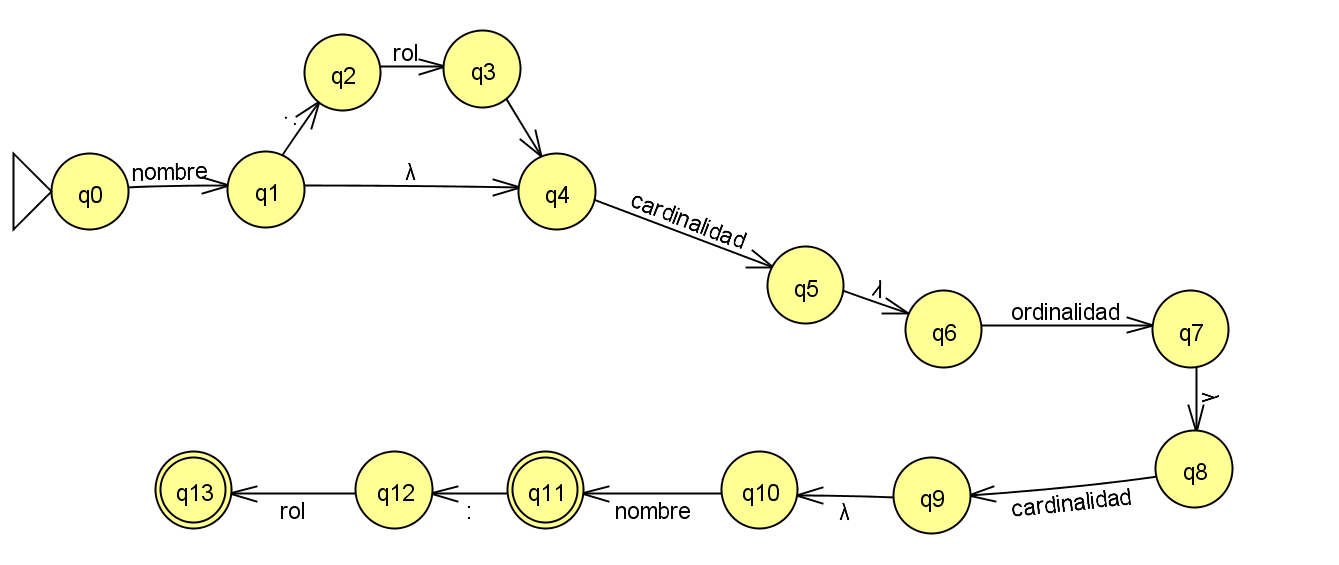
\includegraphics[width=.7\linewidth]{automatas_finitos/relacionDrt.png}
	\caption{Autómata finito - Relación}
	\label{fig:af_relacion}
\end{figure}

\begin{figure}[H]
	\centering
	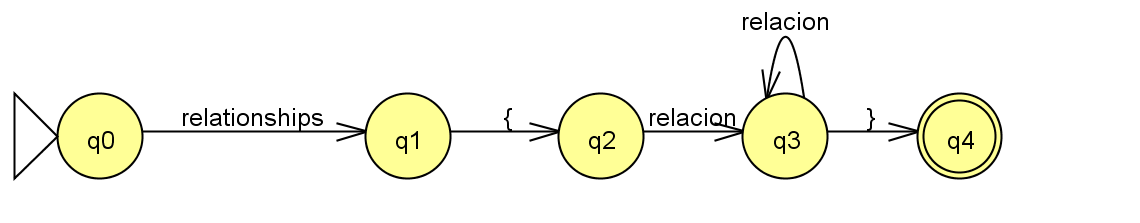
\includegraphics[width=.7\linewidth]{automatas_finitos/relationshipsDrt.png}
	\caption{Autómata finito - Relationships}
	\label{fig:relationships}
\end{figure}

\subsubsection{Analizador Sintáctico}

La notación BNF para las relaciones es la siguiente:

\begin{lstlisting}[caption={BNF - Relationships}, basicstyle=\footnotesize\ttfamily]
  <relationships> ::= "relationships {" <lista-relaciones> "}"
\end{lstlisting}

en donde \texttt{lista-relaciones} se define de la siguiente manera:

\begin{lstlisting}[basicstyle=\footnotesize\ttfamily]
  <lista-relaciones> ::= <relacion> | <lista-relaciones>
\end{lstlisting}

y además se tiene que \texttt{relacion} se define de la siguiente manera:

\begin{lstlisting}[caption={BNF - Relación}, basicstyle=\footnotesize\ttfamily]
	<relacion> ::= <rol-asoc><cardinalidad>
	               <tipo-relacion>
								 <cardinalidad><rol-asoc>
\end{lstlisting}

Se debe realizar la definicion de \texttt{rol-asoc}, \texttt{cardinalidad} y
\texttt{tipo-relacion}.

\subsection*{Definición \texttt{rol-asoc}}
Se procede a definir el significado de \texttt{rol-asoc}, que lo que representa
es el rol que cumple la clase en la relación a establecerce.

\begin{lstlisting}[caption={BNF - Rol},basicstyle=\ttfamily\footnotesize]
  <rol-asoc> ::= <nombre-clase>":"<rol>
\end{lstlisting}

Aquí se tiene que decir que \texttt{nombre-clase} hace referencia a una de las
clases que se tienen en el modelo para el cual se está describiendo la
relación. Luego, se puede definir el significado de \texttt{rol} dentro de las
relaciones. Conceptualmente, el rol pretende darle un nombre personalizado a la
participación de la clase dentro de la relación, este pasará a formar parte (al
momento de la generación del código del modelo) de una de las clases
involucradas en la relación a modo de atributo.

Este último (el rol), no es necesario en la definicion de una relación, dado a
que si este no se encuentra se le asigna un nombre de rol que consistiría en el
nombre de ambas clases involucradas en la relación, en el autómata finito
expuesto en la \texttt{Figura \ref{fig:af_relacion}} se puede ver esto
claramente.

\subsection*{Definición \texttt{cardinalidad}}
\label{sub:cardinalidad}

Dentro de una relación la cardinalidad representa la cantidad con la que
participa la clase en esa asociación con otra clase, de esta manera se pueden
representar cuestiones como:

\begin{displayquote}
	\textit{(...) se pretende que el alumno pueda tener muchas materias (...)}
\end{displayquote}

Aquí es necesario relacionar dos entidades como ser las del \texttt{alumno} y
la de \texttt{materia} para poder representar lo que se solicita, la
cardinalidad en este caso es de \texttt{muchos a muchos}, por el hecho de que,
además de que el alumno pueda tener muchas materias, a las materias pueden
concurrir muchos alumnos, es decir que la materia tambien puede tener asociada
muchos alumnos.

La notación BNF para una relación es la siguiente:

\begin{lstlisting}[caption={BNF - Cardinalidad para una Relación},basicstyle=\footnotesize\ttfamily]
	<cardinalidad> ::= " <digito|`*'> < " |`..' <digito|`*'>> "
\end{lstlisting}

\subsection*{Definicion \texttt{tipo-relacion}}
\label{sub:tiporelacion}

Este elemento, define como se relacionan las clases en una \texttt{relacion}
dada, por ejemplo, puede ser simplemente de \texttt{asociación} o se puede
tener una relación de \texttt{herencia}.

Director maneja estas cuestiones con componentes que buscan el parecido a la
parte gráfica de los diagramas, por este motivo, estos tipos de relación son
literales para cada uno de los tipos que se necesite. A continuación se define
el BNF para el elemento en cuestión.

\begin{lstlisting}[caption={BNF - Tipos de Relación}, basicstyle=\footnotesize\ttfamily]
	<tipo-relacion> ::= <"<--"|"<|-"|"---"|"-|>"|"-->">
\end{lstlisting}

\subsubsection{Derivaciones Relación}
Siguiendo con este componente  con la tendencia de dejar un ejemplo para el
analisis en detalle del componente en cuestión, ahora se toma como sujeto a la
definición de una relación dentro del lenguaje, a continuación, el ejemplo con
el que se estará trabajando:

\begin{lstlisting} [basicstyle=\ttfamily\footnotesize]
  EJEMPLO: nombreClase:nombreRol "1" --- "*" nombreClase2:nombreRol2
\end{lstlisting}

Por cuestiones de espacio y de lo extenso de las derivaciones para los
componentes, se tomaron abreviaciones para los componentes, a continuación
se detalla el significado de cada una de ellos.

\begin{itemize}
  \item \textbf{RA}: rol en la asociacion
  \item \textbf{CA}: cardinalidad
  \item \textbf{TR}: tipo relacion
  \item \textbf{C}: clase
  \item \textbf{SE}: simbolo especial
  \item \textbf{R}: rol
  \item \textbf{D}: delimitador
  \item \textbf{V}: valor
  \item
\end{itemize}


\begin{lstlisting}[basicstyle=\footnotesize\ttfamily, caption={Derivación -
Relación}]
comp-drt -> relacion
comp-drt -> RA     CA    TR CA    RA
comp-drt -> C SE R D V D TR D V D C SE R
comp-drt -> nombreClase SE R D V D TR D V D C SE R
comp-drt -> nombreClase: R D V D TR D V D C SE R
comp-drt -> nombreClase:nombreRol1 D V D TR D V D C SE R
comp-drt -> nombreClase:nombreRol1 " V D TR D V D C SE R
comp-drt -> nombreClase:nombreRol1 "1 D TR D V D C SE R
comp-drt -> nombreClase:nombreRol1 "1" TR D V D C SE R
comp-drt -> nombreClase:nombreRol1 "1"--- D V D C SE R
comp-drt -> nombreClase:nombreRol1 "1"---" V D C SE R
comp-drt -> nombreClase:nombreRol1 "1"---"* D C SE R
comp-drt -> nombreClase:nombreRol1 "1"---"*" C SE R
comp-drt -> nombreClase:nombreRol1 "1"---"*" nombreClase2 SE R
comp-drt -> nombreClase:nombreRol1 "1"---"*" nombreClase2: R
comp-drt -> nombreClase:nombreRol1 "1"---"*" nombreClase2:nombreRol2
\end{lstlisting}

El Árbol Sintáctico corresponediente a la derivación exresada anteriormente es
el siguiente:

\begin{figure}[H]
  \centering
  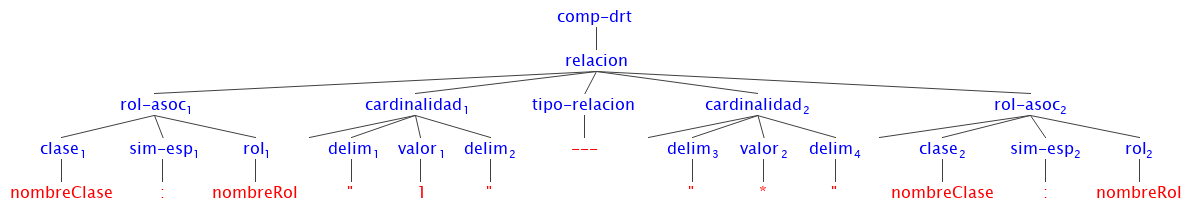
\includegraphics[width=\linewidth]{arboles_sintaxis/5_relacion.png}
  \caption{Árbol Sintáctico - Relación}
  \label{asrelacion}
\end{figure}

